\documentclass[border=4pt,12pt]{standalone}
% House style for redrawn exam diagrams (diagram-v4: 0.4pt lines, filled -latex arrows, fine dashes; stipple and hatching drawn as real dots/lines (no PDF/SVG patterns, so they render in every browser and at any scale); transparent background). Every figure \input's this.
\usepackage{amsmath,amssymb}
\usepackage{txfonts}
\usepackage{pdfrender,xcolor}
% \halo{text}: label on shading. The shading stops just around each letter's outline (a thin knock-out that follows the
% glyphs, like the papers' typesetting), never a box. Owner: "I don't want a box around the text".
\newcommand{\halo}[1]{\leavevmode\rlap{\pdfrender{TextRenderingMode=2,LineWidth=2.2pt,LineJoinStyle=1,StrokeColor=white,FillColor=white}#1}#1}
\usepackage{tikz,pgfplots}
\pgfplotsset{compat=1.18}
\usetikzlibrary{arrows.meta,calc,angles,quotes,patterns,patterns.meta,intersections,positioning,decorations.markings,shapes.geometric}
% Stipple and hatching are drawn as actual dots / lines clipped to the region (path picture), NOT as pattern fills:
% SVG <pattern> fills vanish or blur when browsers scale the image, so the owner could not see the shading.
% Each dot is a 0.72pt square (keeps SVGs small; reads as a dot at print size). Dots sit on one global staggered grid, so neighbouring regions line up.
\makeatletter
\newdimen\ex@x \newdimen\ex@y \newdimen\ex@xa \newdimen\ex@ya \newdimen\ex@xb \newdimen\ex@yb \newcount\ex@row
\def\exam@stipplecolor{black!75}\def\exam@dotr{0.42pt}\def\exam@dotgap{2.5}
\def\ex@rowdots{\ifdim\ex@x<\ex@xb \pgfpathrectangle{\pgfqpoint{\dimexpr\ex@x-0.36pt\relax}{\dimexpr\ex@y-0.36pt\relax}}{\pgfqpoint{0.72pt}{0.72pt}}\advance\ex@x by \exam@dotgap pt\relax\expandafter\ex@rowdots\fi}
\def\exam@stipple{%
  \pgftransformreset% dots are sized in real points even inside scaled pictures
  \pgfpointanchor{path picture bounding box}{south west}\ex@xa=\pgf@x \ex@ya=\pgf@y
  \pgfpointanchor{path picture bounding box}{north east}\ex@xb=\pgf@x \ex@yb=\pgf@y
  \pgfsetfillcolor{\exam@stipplecolor}\pgfmathsetmacro\ex@h{\exam@dotgap/2}%
  \pgfmathtruncatemacro\ex@r{floor(\ex@ya/\ex@h)-1}\ex@row=\ex@r\relax
  \ex@y=\ex@r\dimexpr\ex@h pt\relax
  \loop\ifdim\ex@y<\ex@yb
    \pgfmathtruncatemacro\ex@c{floor(\ex@xa/\exam@dotgap)-1}\ex@x=\ex@c\dimexpr\exam@dotgap pt\relax
    \ifodd\ex@row \advance\ex@x by \ex@h pt\fi
    \ex@rowdots
    \advance\ex@y by \ex@h pt \advance\ex@row by 1
    \ifnum\numexpr\ex@row-(\ex@row/4)*4\relax=0 \pgfusepath{fill}\fi% flush every 4 rows: bounded TeX memory, few clip copies in the SVG
  \repeat\pgfusepath{fill}}
\newdimen\ex@d
\def\exam@hatch#1{% #1 = 1 for /, -1 for \ ; lines 45 degrees, 3pt apart
  \pgftransformreset
  \pgfpointanchor{path picture bounding box}{south west}\ex@xa=\pgf@x \ex@ya=\pgf@y
  \pgfpointanchor{path picture bounding box}{north east}\ex@xb=\pgf@x \ex@yb=\pgf@y
  \ex@d=\dimexpr\ex@yb-\ex@ya\relax \ex@x=\dimexpr\ex@xa-\ex@d\relax
  \loop\ifdim\ex@x<\ex@xb
    \ifnum#1>0 \pgfpathmoveto{\pgfqpoint{\ex@x}{\ex@ya}}\pgfpathlineto{\pgfqpoint{\dimexpr\ex@x+\ex@d\relax}{\ex@yb}}%
    \else \pgfpathmoveto{\pgfqpoint{\ex@x}{\ex@yb}}\pgfpathlineto{\pgfqpoint{\dimexpr\ex@x+\ex@d\relax}{\ex@ya}}\fi
    \advance\ex@x by 4.24pt
  \repeat
  \pgfsetlinewidth{0.4pt}\pgfsetstrokecolor{black}\pgfusepath{stroke}}
\def\examstipple{\exam@stipple}\def\examhatch{\exam@hatch}\def\examsetstipplecolor#1{\def\exam@stipplecolor{#1}}\def\examsetdotgap#1{\def\exam@dotgap{#1}}
\makeatother
% (legacy pattern kept for old files)
% staggered stipple like the NESA papers' dotted shading
\pgfdeclarepatternformonly{exam stipple}{\pgfpointorigin}{\pgfqpoint{2.2pt}{2.2pt}}{\pgfqpoint{2.2pt}{2.2pt}}{%
  \pgfpathcircle{\pgfqpoint{0.55pt}{0.55pt}}{0.42pt}\pgfpathcircle{\pgfqpoint{1.65pt}{1.65pt}}{0.42pt}\pgfusepath{fill}}
\tikzset{
  every picture/.style={line width=0.6pt, >={Latex[length=2mm,width=1.3mm]}},
  curve/.style={line width=0.6pt},
  open arrow/.style={-{Latex[length=2mm,width=1.3mm]}},  % owner: filled -latex heads everywhere, no open chevrons
  aux/.style={dash pattern=on 2pt off 1.5pt, line width=0.6pt},
  shade/.code={\def\exA{#1}\def\exB{none}\ifx\exA\exB\else\pgfkeysalso{fill=black!18}\fi},
  shade/.default=on,
  shade dots/.style={fill=none, path picture={\examstipple}},
  stipple color/.code={\examsetstipplecolor{#1}},
  stipple gap/.code={\examsetdotgap{#1}},
  shade dense dots/.style={fill=none, stipple gap=1.6, path picture={\examstipple}},
  shade hatch/.style={fill=none, path picture={\examhatch{1}}},
  shade hatch reverse/.style={fill=none, path picture={\examhatch{-1}}},
  shade solid/.style={fill=black},
  pt/.style={circle, fill, inner sep=1.1pt},
  open pt/.style={circle, draw, fill=white, inner sep=1.1pt},
}
\pgfplotsset{
  exam axes/.style={axis lines=middle, axis line style={->}, xlabel={$x$}, ylabel={$y$},
    xlabel style={anchor=west}, ylabel style={anchor=south}, tick label style={font=\small},
    every axis plot/.append style={line width=0.6pt, black}, samples=200, clip=false,
    enlargelimits=false, axis on top},
}

\begin{document}
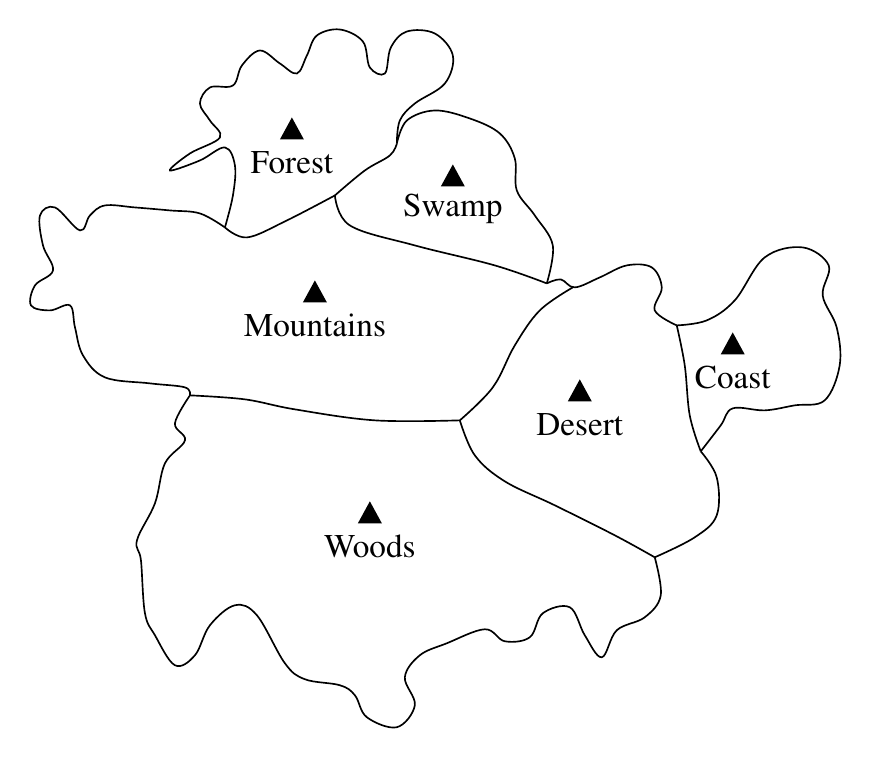
\begin{tikzpicture}[x=0.0127cm,y=-0.0127cm]
  % outer coastline, clockwise from the forest/mountain corner
  \draw plot[smooth, tension=0.6] coordinates {(230,212) (238,180) (240,150) (230,132) (205,145) (175,155) (195,138) (225,122) (215,105) (205,88) (215,72) (238,70) (247,50) (265,35) (285,48) (302,58) (312,40) (322,20) (345,14) (368,26) (375,52) (390,58) (396,32) (412,16) (440,18) (458,40) (450,68) (420,88) (405,105) (402,128)};
  \draw plot[smooth, tension=0.6] coordinates {(402,128) (412,105) (440,95) (475,103) (505,118) (520,143) (522,175) (540,200) (558,230) (552,268)};
  \draw plot[smooth, tension=0.6] coordinates {(552,268) (566,264) (580,272) (605,262) (632,250) (657,252) (667,272) (660,295) (682,310)};
  \draw plot[smooth, tension=0.6] coordinates {(682,310) (712,305) (740,285) (770,242) (808,232) (834,250) (828,280) (842,312) (845,350) (830,385) (800,390) (770,395) (738,393) (726,410) (706,436)};
  \draw plot[smooth, tension=0.6] coordinates {(706,436) (722,462) (722,500) (700,522) (660,542)};
  \draw plot[smooth, tension=0.6] coordinates {(660,542) (666,580) (650,602) (622,615) (607,642) (590,620) (575,592) (548,598) (535,622) (510,626) (490,614) (452,628) (425,640) (410,662) (420,690) (402,712) (372,702) (360,680) (345,670) (310,664) (290,648) (262,600) (240,590) (215,610) (200,640) (180,650) (160,620) (150,598) (146,545) (142,525) (160,488) (170,448) (190,425) (180,408) (195,380)};
  \draw plot[smooth, tension=0.6] coordinates {(195,380) (190,372) (155,368) (110,362) (88,340) (80,312) (75,290) (55,295) (36,290) (40,270) (58,255) (48,230) (45,200) (60,192) (85,215) (95,200) (110,190) (140,192) (175,195) (205,198) (230,212)};
  % internal borders
  \draw plot[smooth, tension=0.6] coordinates {(230,212) (252,222) (290,206) (340,180)};
  \draw plot[smooth, tension=0.6] coordinates {(340,180) (370,155) (395,140) (402,128)};
  \draw plot[smooth, tension=0.6] coordinates {(340,180) (355,210) (420,230) (500,250) (552,268)};
  \draw plot[smooth, tension=0.6] coordinates {(195,380) (250,384) (300,394) (380,405) (465,405)};
  \draw plot[smooth, tension=0.6] coordinates {(465,405) (498,372) (520,330) (545,295) (578,272)};
  \draw plot[smooth, tension=0.6] coordinates {(682,310) (690,350) (695,400) (706,436)};
  \draw plot[smooth, tension=0.6] coordinates {(465,405) (480,440) (510,466) (560,490) (620,520) (660,542)};
  % region markers and names
  \foreach \x/\y/\t in {297/113/Forest, 458/160/Swamp, 320/276/Mountains, 585/375/Desert, 738/328/Coast, 375/497/Woods} {
    \fill (\x-12,\y+11) -- (\x+12,\y+11) -- (\x,\y-11) -- cycle;
    \node[font=\large] at (\x,\y+34) {\t};}
\end{tikzpicture}
\end{document}